\documentclass[11pt,letterpaper]{article}
\usepackage[margin=0.6in]{geometry}
\usepackage{amsmath,amssymb}
\usepackage{tikz}
\usetikzlibrary{arrows.meta,positioning}
\usepackage{xcolor}
\usepackage{fontawesome5}
\usepackage{tcolorbox}
\usepackage{multicol}
\usepackage{enumitem}
\usepackage{hyperref}

\definecolor{primaryblue}{RGB}{41, 98, 255}
\definecolor{accentgreen}{RGB}{0, 150, 136}
\definecolor{warnorange}{RGB}{255, 152, 0}
\definecolor{lightgray}{RGB}{245, 245, 245}

\tcbset{
    conceptbox/.style={colback=primaryblue!5, colframe=primaryblue, boxrule=1pt, arc=3pt, left=5pt, right=5pt, top=5pt, bottom=5pt},
    formulabox/.style={colback=lightgray, colframe=gray!50, boxrule=0.5pt, arc=2pt, left=5pt, right=5pt, top=3pt, bottom=3pt},
    warningbox/.style={colback=warnorange!10, colframe=warnorange, boxrule=1pt, arc=3pt, left=5pt, right=5pt, top=5pt, bottom=5pt},
    appbox/.style={colback=accentgreen!5, colframe=accentgreen, boxrule=1pt, arc=3pt, left=5pt, right=5pt, top=5pt, bottom=5pt}
}

\pagestyle{empty}
\setlength{\parindent}{0pt}
\setlist[itemize]{leftmargin=*, itemsep=1pt, topsep=2pt}

\begin{document}

\begin{center}
{\LARGE\bfseries\color{primaryblue} Chapter 2: Probability \& Statistics}\\[3pt]
{\large Reasoning Under Uncertainty}
\end{center}
\vspace{-5pt}
\hrule height 2pt
\vspace{8pt}

\begin{multicols}{2}

\begin{tcolorbox}[conceptbox, title={\faLightbulb\ Key Concepts}]
\begin{itemize}
    \item \textbf{Random Variable}: Maps outcomes to numbers
    \item \textbf{PDF/PMF}: Probability density/mass function
    \item \textbf{Expectation}: Average value, $\mathbb{E}[X]$
    \item \textbf{Variance}: Spread around mean, $\text{Var}(X)$
    \item \textbf{Bayes' Theorem}: Update beliefs with evidence
    \item \textbf{MLE}: Find parameters that maximize likelihood
\end{itemize}
\end{tcolorbox}

\begin{tcolorbox}[formulabox, title={\faCalculator\ Core Formulas}]
\textbf{Bayes' Theorem:}
\[ P(A|B) = \frac{P(B|A) \cdot P(A)}{P(B)} \]

\textbf{Expectation:}
\[ \mathbb{E}[X] = \sum_x x \cdot P(X=x) \]

\textbf{Gaussian PDF:}
\[ p(x) = \frac{1}{\sqrt{2\pi\sigma^2}} e^{-\frac{(x-\mu)^2}{2\sigma^2}} \]

\textbf{MLE:}
\[ \hat{\theta} = \arg\max_\theta \prod_{i=1}^{n} p(x_i | \theta) \]
\end{tcolorbox}

\columnbreak

\begin{center}
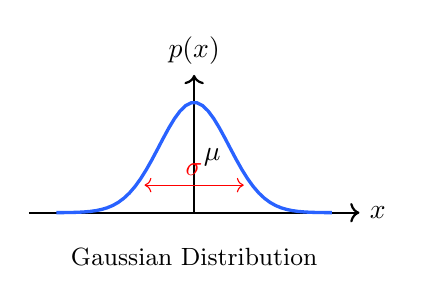
\begin{tikzpicture}[scale=0.7]
    % Gaussian curve
    \draw[->,thick] (-3,0) -- (3,0) node[right] {$x$};
    \draw[->,thick] (0,0) -- (0,2.5) node[above] {$p(x)$};

    \draw[primaryblue, very thick, domain=-2.5:2.5, samples=50]
        plot (\x, {2*exp(-\x*\x/0.8)});

    % Mean and std dev
    \draw[dashed] (0,0) -- (0,2) node[midway,right] {$\mu$};
    \draw[<->,red] (-0.9,0.5) -- (0.9,0.5) node[midway,above] {$\sigma$};

    \node at (0,-0.8) {\small Gaussian Distribution};
\end{tikzpicture}
\end{center}

\begin{tcolorbox}[appbox, title={\faRobot\ ML Applications}]
\begin{itemize}
    \item \textbf{Classification}: Softmax outputs probabilities
    \item \textbf{Naive Bayes}: Spam filtering, text classification
    \item \textbf{Gaussian Processes}: Probabilistic regression
    \item \textbf{VAEs}: Latent variable models with priors
    \item \textbf{Dropout}: Approximate Bayesian inference
\end{itemize}
\end{tcolorbox}

\begin{tcolorbox}[warningbox, title={\faExclamationTriangle\ Common Pitfalls}]
\begin{itemize}
    \item \textbf{Base rate fallacy}: Ignoring prior probabilities
    \item Confusing $P(A|B)$ with $P(B|A)$
    \item MLE can \textbf{overfit} with small data
    \item Assuming independence when variables are correlated
\end{itemize}
\end{tcolorbox}

\end{multicols}

\vspace{5pt}
\hrule
\vspace{5pt}

\begin{center}
\faGithub\ \textbf{Notebook}: \url{https://github.com/vijaygwu/math-powers-ai/blob/main/notebooks/ch02_probability.ipynb}
\end{center}

\end{document}
